\section{Application to Collider Data}\label{sec:ResFit:DataDriven}

In the following, the resolution measurement in Collider data is
discussed.

\qsec{sec:ResFit:Asym:SimpleFit} is devoted to the comparison of the performance of a
binned and an unbinned fit of the dijet asymmetry.
The completely analogue case is demonstrated in
\qsec{sec:ResFit:Asym:SimpleFit} where the likelihood is simplified by replacing the spectrum
with the assumption \mbox{$\pttrue = \ptave$}.
Since the unbinned fit is more sensitive to non-Gaussian tails, an outlier
suppression technique is introduced.
In \qsec{sec:ResFit:Asym:FullFit}, the full dijet pdf, including an assumption for the
spectrum and a description of selection biases, is finally used to fit the asymmetry;
the spectrum is also used to derive a better estimator for \ptgen.

As discussed in \qsec{sec:ResFit:AddJets}, additional jets in the events, e.g. from soft gluon radiation, as
well as out-of-cone effects during the jet clustering bias the dijet asymmery and have to be
corrected for when measuring the resolution.
The contributions to the bias are investigated in detail in \qsec{sec:ResFit:AddJets:Contributions} and
in \qsec{sec:ResFit:AddJets:Extrapolation} a correction method is presented using an extrapolation of
the resolution to the ideal two jet case.


\subsection{Fit of the Dijet Asymmetry}\label{sec:ResFit:Asym}

The dijet asymmetry is defined as
\begin{equation}\label{eq:ResFit:Asymmetry}
  A = \frac{\pti{1'}-\pti{2'}}{\pti{1'}+\pti{2'}},
\end{equation}
where \pti{1'} and \pti{2'} refer to the randomly ordered transverse momenta of the
leading two jets in an event.
In case of events with exactly two jets of same particle level jet
transverse momentum \pt and Gaussian response, the width $\sigma(A)$ of the asymmetry distribution is
related to the jet \pt resolution $\sigma$ by
\begin{equation}
  \label{eq:ResFit:ResFromAsym}
  \sigma(A) = \frac{1}{\sqrt{2}}\frac{\sigma}{\pt} \; .
\end{equation}


\subsubsection{Simple Maximum Likelihood Fit and Outlier Treatment}\label{sec:ResFit:Asym:SimpleFit}

If the spectrum $f$ in the dijet pdf~\qeq{eq:ResFit:DijetPdfTransformed} is replaced by \mbox{$f(\pttrue)  = \delta\left(\pttrue - \ptave\right)$}, i.e. assuming \mbox{$\pttrue = \ptave$}, 
\qeq{eq:ResFit:DijetPdfTransformed} simplifies to
\begin{equation}
\label{eq:ResFit::DijetPdfTransformed:Simple}
  g_{\sigma'}\left(\Delta\pt\right) \propto
  \e^{-\frac{1}{2}\left(\frac{\Delta\pt}{\sigma'}\right)^{2}}, 
\end{equation}
with \mbox{$\sigma' = \sigma/\sqrt{2}$}.
This corresponds to the pdf of the asymmetry in the event, assuming
Gaussian response.

In real data, however, there are non-Gaussian tails biasing the fit of the asymmetry.
In case of a binned fit of the histogram, the influence of the tails is suppressed by
fitting only the bulk of the distribution, defined as two standard deviations around the mean.
In case of the unbinned fit, it is not as straight
forward to select only the bulk events.
This can be achieved, however, with an iterative procedure by restricting
the allowed range of $\Delta\pt$.
As observed in data and MC simulation (\fixme{reference to plot}), tails start to appear for \mbox{$|\Delta\pt| > 2\sigma'$}.
Hence, the unbinned fit is performed only for events with \mbox{$|\Delta\pt| < 2\sigma'$}.
In order to preserve unitarity of the dijet pdf, the normailisation
of~\qeq{eq:ResFit::DijetPdfTransformed:Simple} is adapted accordingly.
\fixme{State complete pdf in Appendix}

The threshold on $|\Delta\pt|$ in the above choice is proportional to $\sigma'$, which is the fitted parameter, and would be varied accordingly during the maximisation.
This, however, biases the result towards smaller \fixme{???} values.
Therefore the threshold is kept fixed and the maximisation is iterated
four times, leading to an unbiased result.

\begin{figure}[ht]
  \label{fig:ResFit:Asym:Simple}
  \centering
  \begin{tabular}{cc}
    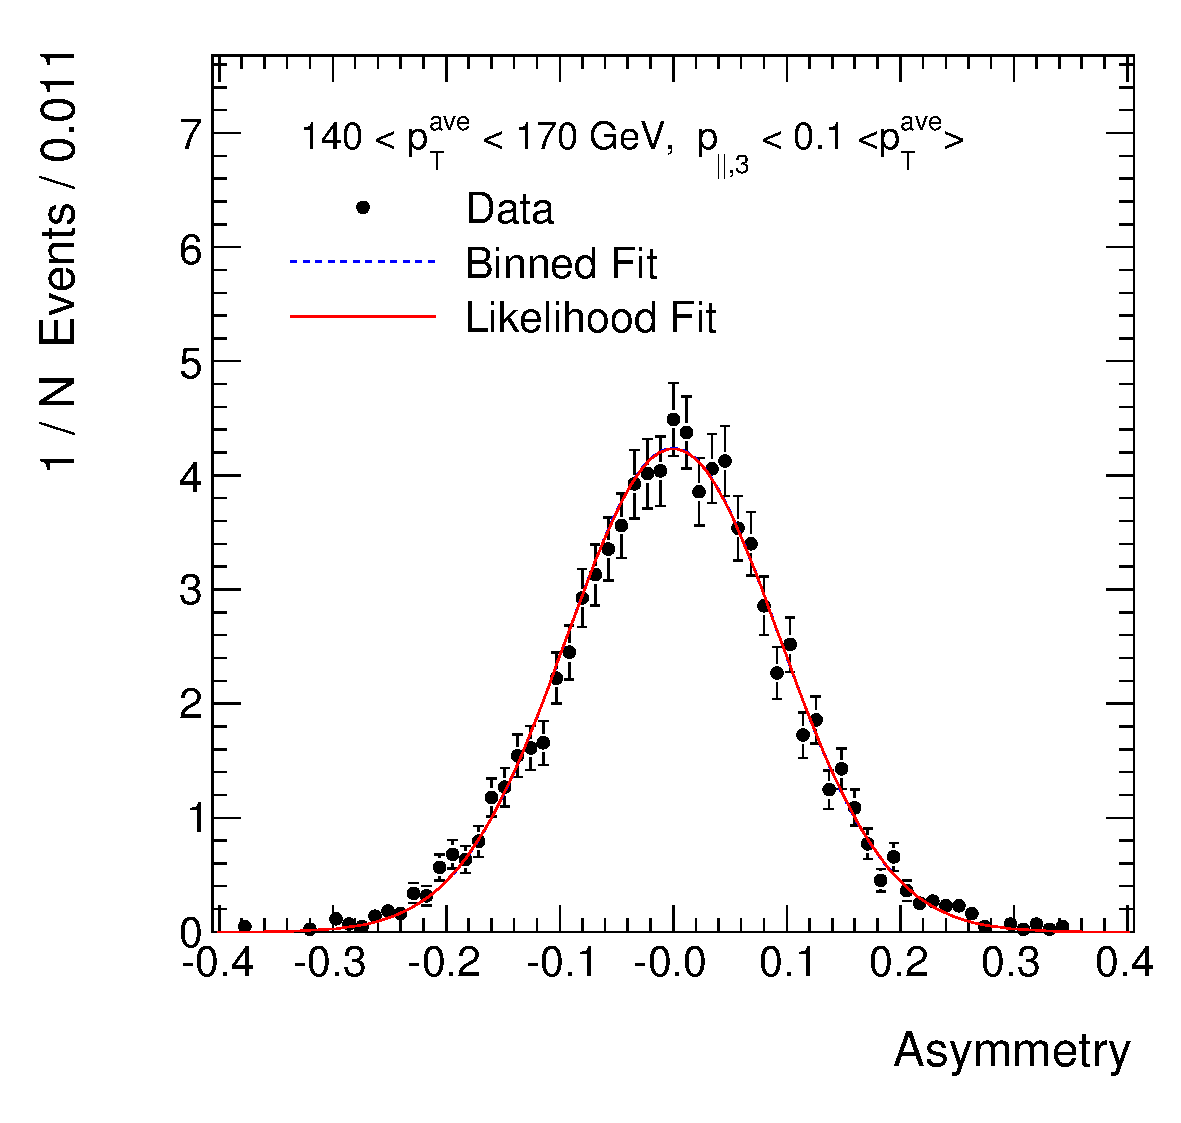
\includegraphics[width=0.45\textwidth]{figures/MaxLikeSimple_Data132440-144011_Eta00-13_PtAsymmetry_PtBin4_Pt3Cut3} &
    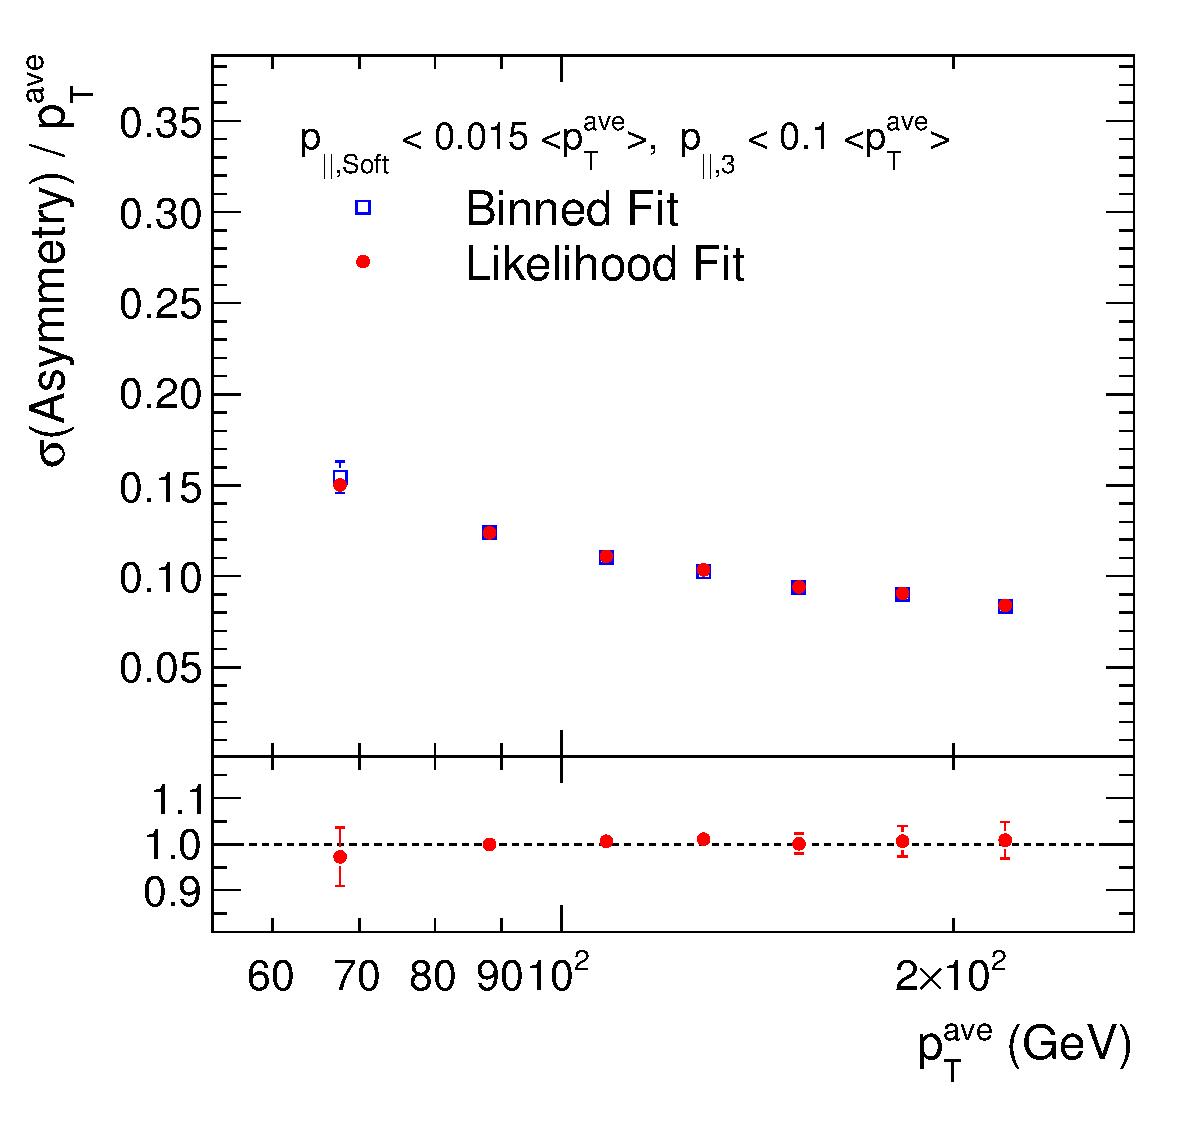
\includegraphics[width=0.45\textwidth]{figures/MaxLikeSimple_Data132440-144011_Eta00-13_PtAsymmetryWidthBottomRatio_Pt3Cut3} \\
\end{tabular}
  \caption{(\textit{Left}) Dijet asymmetry distribution measured in
    Collider data (circles) for \mbox{$\ppi{3} < 0.1\cdot\mean{\ptave}$} and \mbox{$\ppi{\text{Soft}} < 0.015\cdot\mean{\ptave}$} in the \mbox{$140 < \ptave < 170\gev$} bin.
    It is well described by the prediction (solid line) from the
    simplified unbinned maximum likelihood fit and there is good agreement to a direct binned
    fit (dashed line) of the histogram.
    Note that both lines lie in fact on top of each other.
    (\textit{Right}) Width of the asymmetry distributions from
    Collider data in different \ptave bins from binned Gaussian fits to the
    histograms (open squares) in comparison to the predictions from
    the unbinned fit (solid circles).}
\end{figure}

The asymmetry distribution measured in Collider data for \mbox{$140 < \ptave < 170\gev$}, \mbox{$\ppi{3} < 0.1\cdot\mean{\ptave}$}, and \mbox{$\ppi{\text{Soft}} < 0.015\cdot\mean{\ptave}$} is shown in \qsubfig{fig:ResFit:Asym:Simple}{left}.
It is well described by the result of the discussed simplified unbinned fit, i.e. a Gaussian with width $\sigma'$, and there is good agreement to a direct binned fit of the histogram.
In \qsubfig{fig:ResFit:Asym:Simple}{right}, the widths $\sigma'$ measured in different \ptave bins with the unbinned technique are further compared to the results of binned fits.
Again, there is good agreement.

In conclusion, the simplified unbinned likelihood fit of the asymmetry performs equally to a binned fit of corresponding histogram.



\subsubsection{Full Maximum Likelihood Fit Including the Spectrum and Description of the Selection Bias}\label{sec:ResFit:Asym:FullFit}

In the following, the extension of the dijet pdf with an assumption for the particle level jet \pt cross section $f$ is discussed.
With the choice of coordinates~\qeq{eq:ResFit:TransformedCoordinates}, this corresponds to multiplying a pdf for the measured \ptave,
\begin{equation*}
\label{eq:ResFit::DijetPdfTransformed:Simple}
  g_{\sigma'}\left(\ptave\right) \propto
  \int\dif{\pttrue}\;f\left(\pttrue\right)\cdot
  \e^{-\frac{1}{2}\left(\frac{\ptave - \pttrue}{\sigma'}\right)^{2}} \, , 
\end{equation*}
resulting in~\qeq{eq:ResFit:DijetPdfTransformed}.
As mentioned before, the spectrum is taken from the MC simulation (\qsubfig{fig:ResFit:Asym:Spectrum}{left}) and not modified during the fit.
The resulting systematic uncertatinties have to be evaluated.

By this extension, additionally a description of biases in the event selection can be included into the likelihood.
Binning in (measured) \ptave causes migration effects at the edges of the selected \ptave range due to the finite jet \pt resolution:
there are jets that fluctuate either into or out of the selected interval.
This is illustrated in \qsubfig{fig:ResFit:Asym:Spectrum}{right} with simulated data using the MC truth information.
Additionally, because of the steeply falling dijet \pt spectrum, there are more jets that fluctuate high than jets that fluctuate low in \pt and the selected sample is therefore biased towards jets of lower \ptgen that fluctuated high in the detector.

\begin{figure}[ht]
  \label{fig:ResFit:Asym:Spectrum}
  \centering
  \begin{tabular}{cc}
    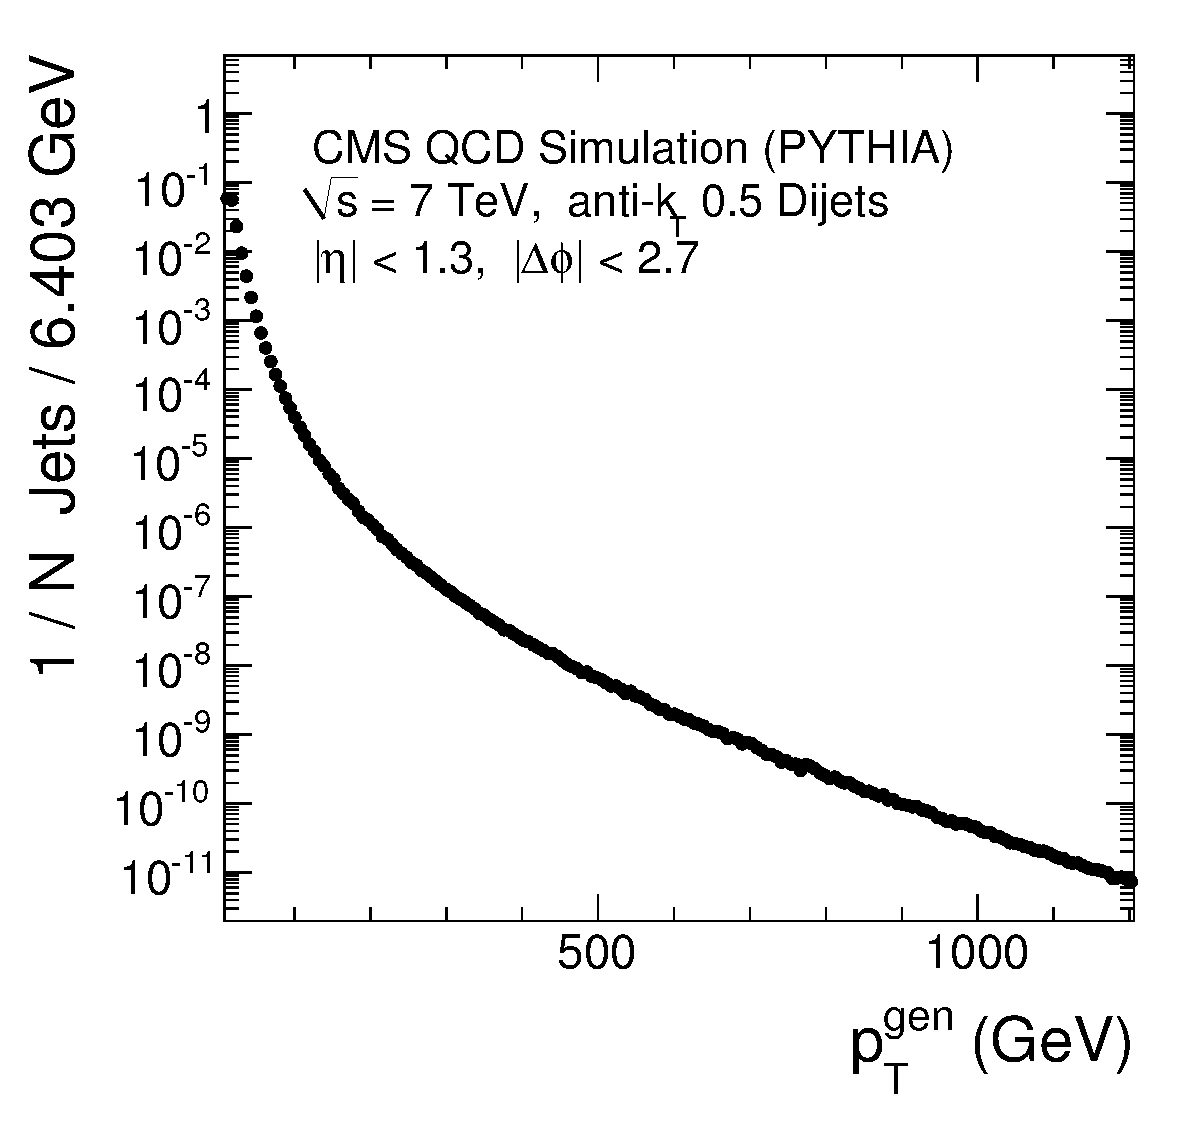
\includegraphics[width=0.45\textwidth]{figures/ExampleSpectrum} &
    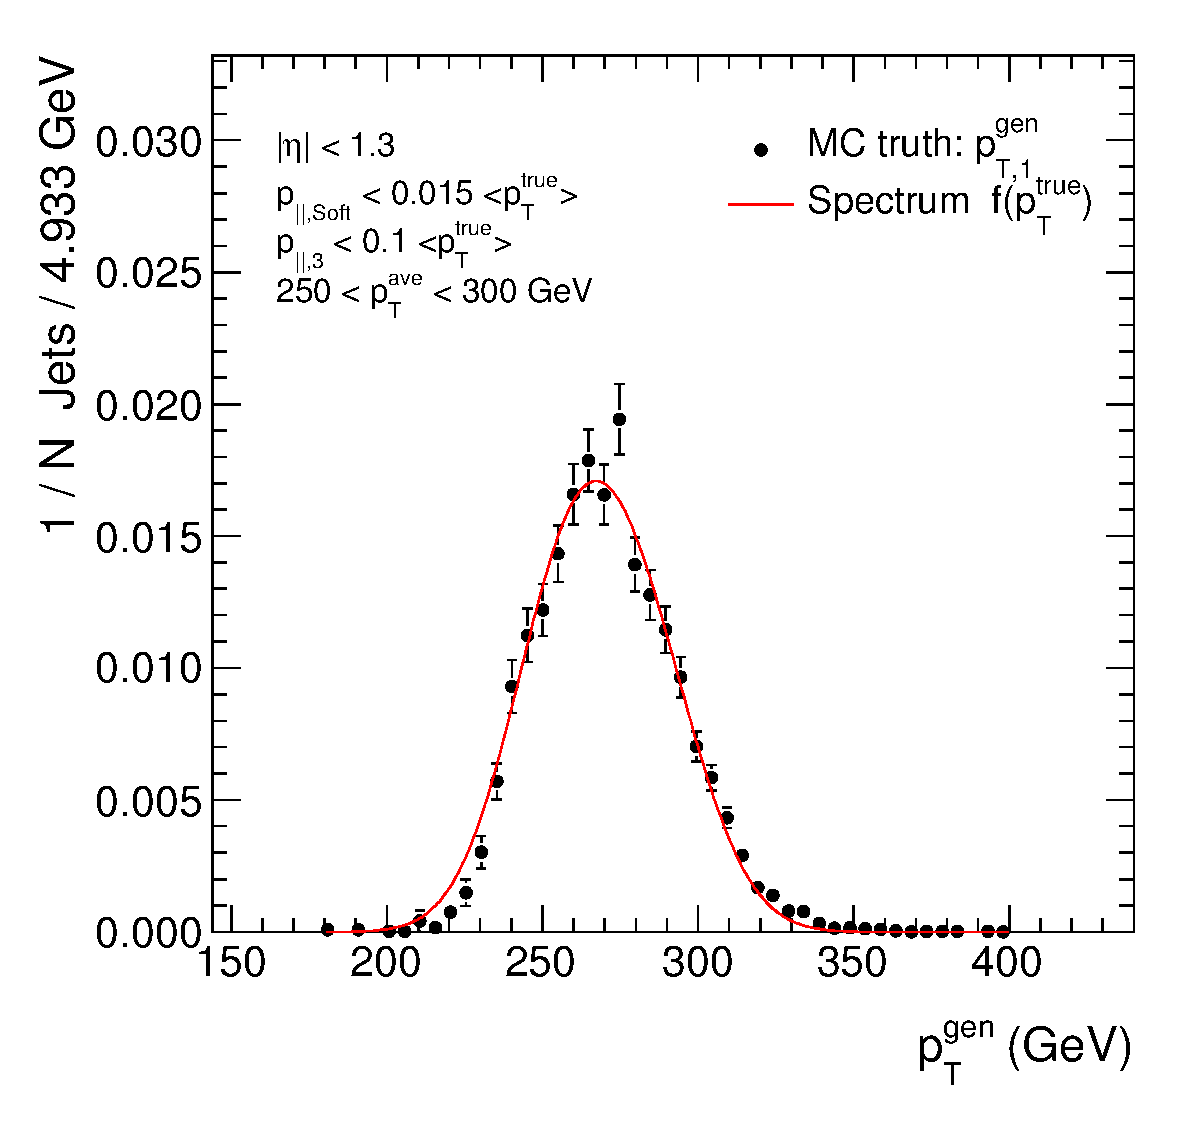
\includegraphics[width=0.45\textwidth]{figures/MaxLike_Eta00-13_SpectrumJet1_PtBin7}\\
 \end{tabular}
  \caption{(\textit{Left}) Dijet \ptgen spectrum from the MC simulation.
    Per selected event, the \ptgen of both the leading jets has been filled into the histogram.
    A linear interpolation of this histogram is used as the particle level differential jet cross section in~\qeq{eq:ResFit:Asym:ModifiedSpectrum}.
    (\textit{Right}) \ptgen spectrum (circles) of the selected dijet events in the \mbox{$250 < \ptave < 300\gev$} bin.
    It is well described by the modified cross section $f$ in~\qeq{eq:ResFit:Asym:ModifiedSpectrum} (solid line).}
\end{figure}

The dijet pdf~\qeq{eq:ResFit:DijetPdfTransformed} is modified to describe the
\ptave selection and hence avoid biasing the measured resolution.
First, the allowed range of \ptave is considered in the normalisation. \fixme{Reference to Appendix}
Second, the \pttrue pdf is extended to incorporate the migration effects:
\begin{equation}
  \label{eq:ResFit:Asym:ModifiedSpectrum}
  f\left(\pttrue\right) = \frac{1}{\mathcal{N}_{f}}
  f_{0}\left(\pttrue\right) \int^{\ptavemax}_{\ptavemin}\dif{x}\;\mathcal{G}\left(x|\sigma',\pttrue\right) \, ,
\end{equation}
Here, $f_{0}$ denotes the underlying particle level jet \pt spectrum \qsubfig{fig:ResFit:Asym:Spectrum}{left}\footnote{The actual probability densities are evaluated using a linear interpolation of the histogram.} and $\mathcal{G}$ is a Gaussian of width \mbox{$\sigma' = \sigma/\sqrt{2}$}, i.e. the pdf of \ptave for a given \pttrue.
Equation~\qeq{eq:ResFit:Asym:ModifiedSpectrum} is validated using simulate data:
the \ptgen spectrum of selected dijet events is well described by $f(\pttrue)$ as demonstrated in \qsubfig{fig:ResFit:Asym:Spectrum}{right}.
This extension to $f$ depends solely on the fitted parameter $\sigma'$ and does not introduce any new dependencies on the MC simulation.



\subsection{Influence of Additional Hadronic Activity and Hadronisation Effects}\label{sec:ResFit:AddJets}

\subsubsection{Contributions to the Dijet Asymmetry}\label{sec:ResFit:AddJets:Contributions}

In \qsubfig{fig:ResFit:AddJets:Bias}{left}, the standard deviations of
the asymmetry distribution, multiplied by a factor $\sqrt{2}$,
are shown for various \ptgen bins for simulated dijets.
According to~\qeq{eq:ResFit:ResFromAsym} these should corresond to the
jet \pt resolution.
However, they are greater than the MC truth resolutions for the
following reasons.
The dijet asymmetry~\qeq{eq:ResFit:Asymmetry} is defined under the assumption of exactly two jets which are balanced in transverse momentum at particle level.
Additional jet acitivity in the events, e.g. from soft gluon
radiation, causes an imbalance of the leading two jets and hence
broadens the measured asymmetry distribution.

\begin{figure}[ht]
  \label{fig:ResFit:AddJets:Bias}
  \centering
  \begin{tabular}{cc}
    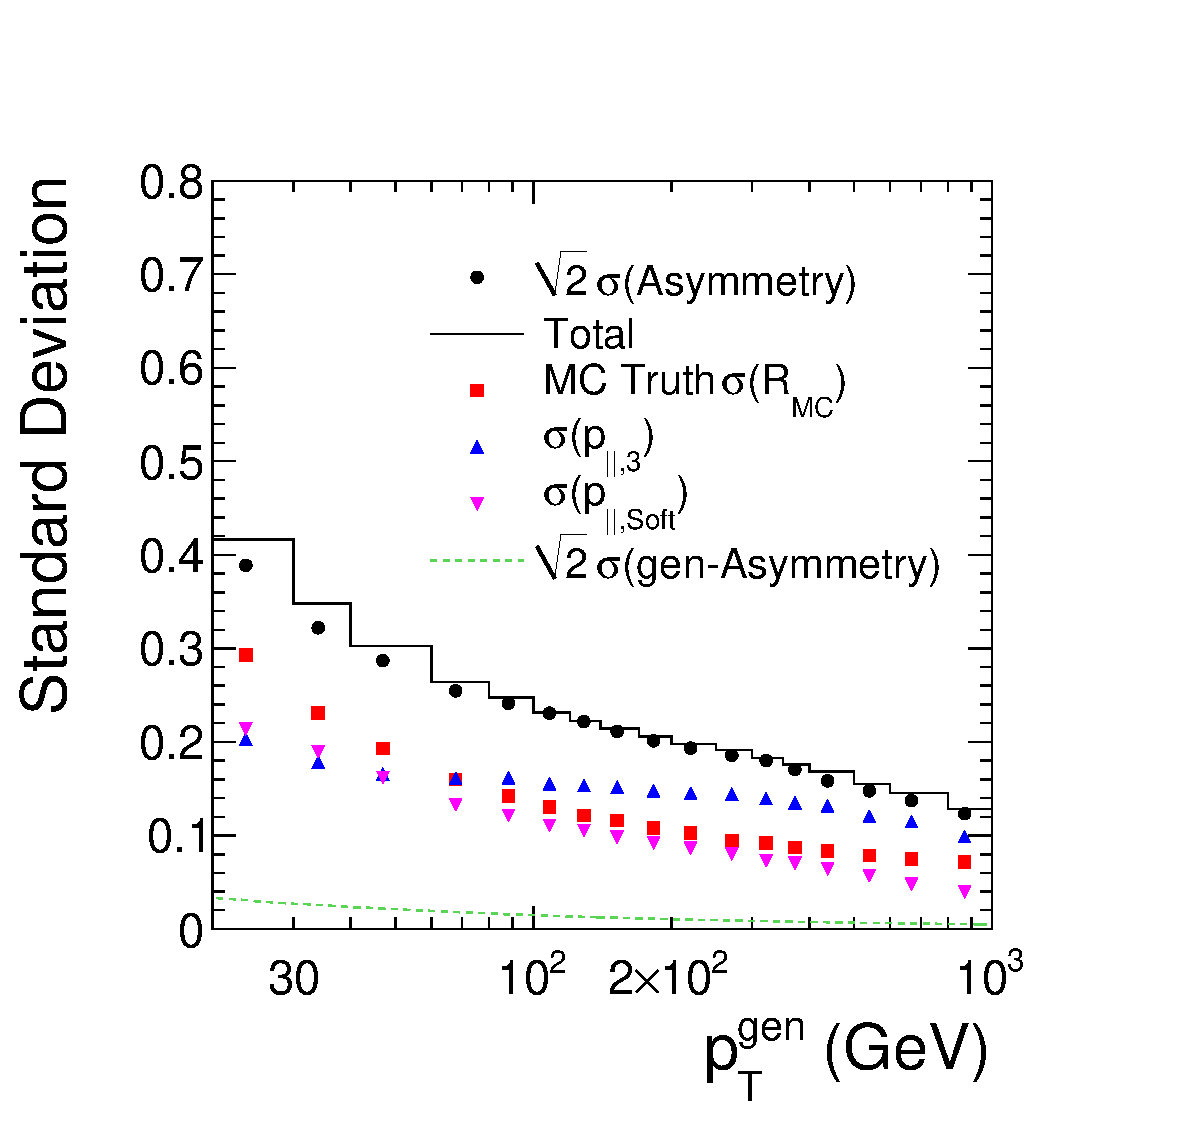
\includegraphics[width=0.45\textwidth]{figures/Spring10QCDDiJet_ParallelComponent_hParallelContributions} &
    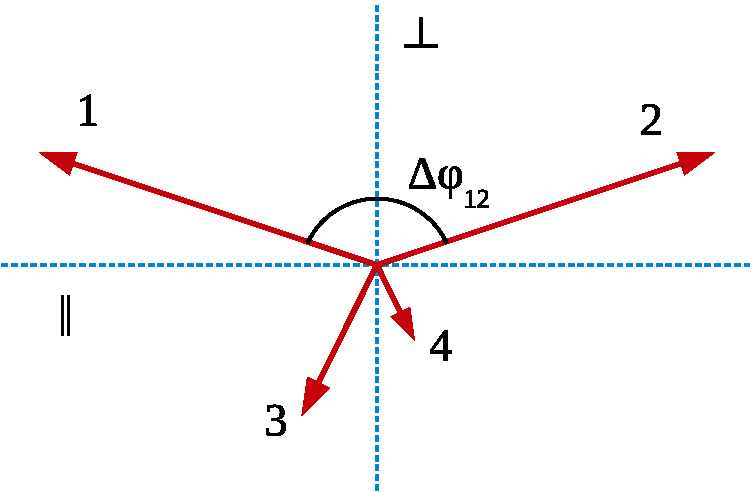
\includegraphics[width=0.45\textwidth]{figures/Sketch_Projections}
  \end{tabular}
  \caption{\mbox{$|\Delta\phi_{12}| > 2.7$} (\textit{Left}) Definition of the dijet axis $\phi_{||}$, the direction normal to the
    angle bisector of the leading two jets in the transverse plane.
    Additional jets with \pt components along $\phi_{||}$ will cause
    a \pt imbalance of the particle jets and bias the measured
    resolution towards larger values.
    (\textit{Right}) Gaussian resolutions \mbox{$\sigma/\mean{\pttrue}$} measured with the unbinned
    fit in Collider data for \mbox{$140 < \ptave < 170\gev$} and different \ppi{3}
    thresholds after suppression of additional soft jet activity along
    $\phi_{||}$. 
    \mbox{$\sigma/\mean{\pttrue}$} on \ppi{3} is linearly
    extrapolated to the case of an ideal dijet event.
  }
\end{figure}

As illustrated in \qsubfig{fig:ResFit:AddJets:Bias}, not the
absolute \pt of the additional jets actually affects the balance, but rather the component along the dijet axis, $\phi_{||}$, defined as the direction normal to the angle bisector of the leading two jets.
The parallel \pt components of the third and all further
(\textit{soft}) jets may be defined as
\begin{align}
  \begin{split}
    \ppi{3}               & =  |\pti{3}\cos(\phi_{3}-\phi_{||})| \\
    \ppi{\text{Soft}} & =  |\sum_{i>3}\pti{i}\cos(\phi_{i}-\phi_{||})| \,.
  \end{split}
\end{align}
The total standard deviation of the measured dijet asymmetry
distribution (multiplied by $\sqrt{2}$) can hence be understood as the
quadratic sum of the underlying dijet asymmetry due to the jet \pt response,
$\sigma(R_{\text{MC}})$, and the standard deviations of the \pp
distributions, $\sigma(\ppi{3})$ and
$\sigma(\ppi{\text{Soft}})$,
\begin{equation}
  \label{eq:ResFit:TotalAsym}
  \text{Total} = \sigma(R_{\text{MC}}) \oplus \sigma(\ppi{3}) \oplus
  \sigma(\ppi{\text{Soft}}) \oplus \sqrt{2}\sigma(A^{\text{gen}}) \,.
\end{equation}

The transverse momentum balance assumed for the particle level jets
actually takes place at parton level.
Owing to the fragmentation and hadronisation, fluctuations in the
fraction of energy of the original partons clustered into jets are
expected (out-of-cone).
This is an additional process introducing an imbalance in the
dijet events and the contribution is estimated using the \ptgen
asymmetry, $A^{\text{gen}}$, in perfect
two jet events.
The standard deviation $\sqrt{2}\sigma(A^{\text{gen}})$ is also added in quadrature to
$\sigma(R_{\text{MC}})$, hence the last term in~\qeq{eq:ResFit:TotalAsym}.

The dijet pdf~\qeq{eq:ResFit:DijetPdf} has been shown to be equivalent
to the asymmetry and has also been defined under the assumption of \pt
balance at particle jet level.
Hence it will be biased by the same effects.



\subsubsection{Correction for Additional Hadronic Activity}\label{sec:ResFit:AddJets:Extrapolation}

In order to compensate for the presence of additional jets,
events are selected\footnote{The resulting selection bias is incorporated in the dijet pdf as
before, comp. \qsec{sec:ResFit:Asym:FullFit}.} in reasonably small bins of \ptave.
Per bin, the \pp components of the third and all further jets are restricted to
\begin{align}
  \label{eq:ResFit:ThirdJetSelection}
  \begin{split}
    \ppi{3}                & < z\cdot\mean{\pttrue} \\
    \ppi{\text{Soft}}  & < 0.015\cdot\mean{\pttrue},
 \end{split}
\end{align}
where $\mean{\pttrue}$ is the mean particle level jet \pt in that bin
as estimated from the assumed spectrum
$f$ in~\qeq{eq:ResFit:Asym:ModifiedSpectrum}.
Several sets of dijet events are selected, each with a different
threshold $z$ of \ppi{3}, and the mean Gaussian response with \pt
independent resolution $\sigma$ is measured by maximising the dijet
likelihood~\qeq{eq:ResFit:Likelihood} w.r.t. $\sigma$.
The dependence of the jet \pt resolution on the threshold $z$ is
clearly visible in \qsubfig{fig:ResFit:AddJets:Corr}{right}.
In order to extrapolate the measurement to the case of a two jet only
event, the \mbox{$\sigma/\mean{\pttrue}$} are fitted with a linear
function and the $y$ axis intercept is used as the unbiased jet \pt
resolution.

\begin{figure}[ht]
  \label{fig:ResFit:AddJets:Corr}
  \centering
  \begin{tabular}{cc}
    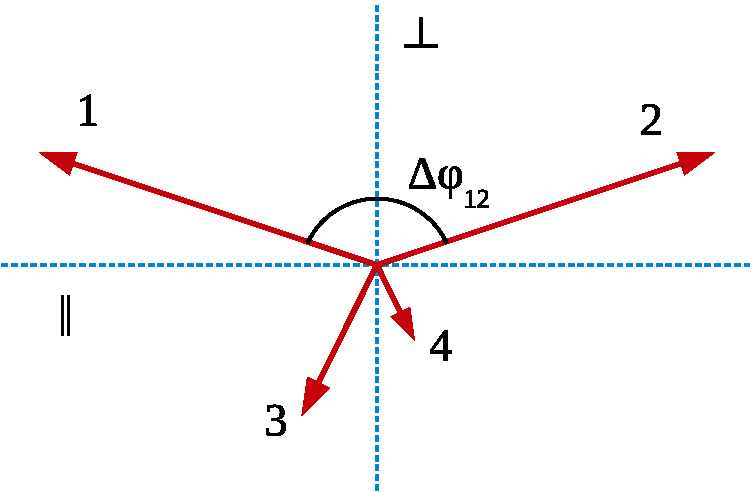
\includegraphics[width=0.45\textwidth]{figures/Sketch_Projections}
    %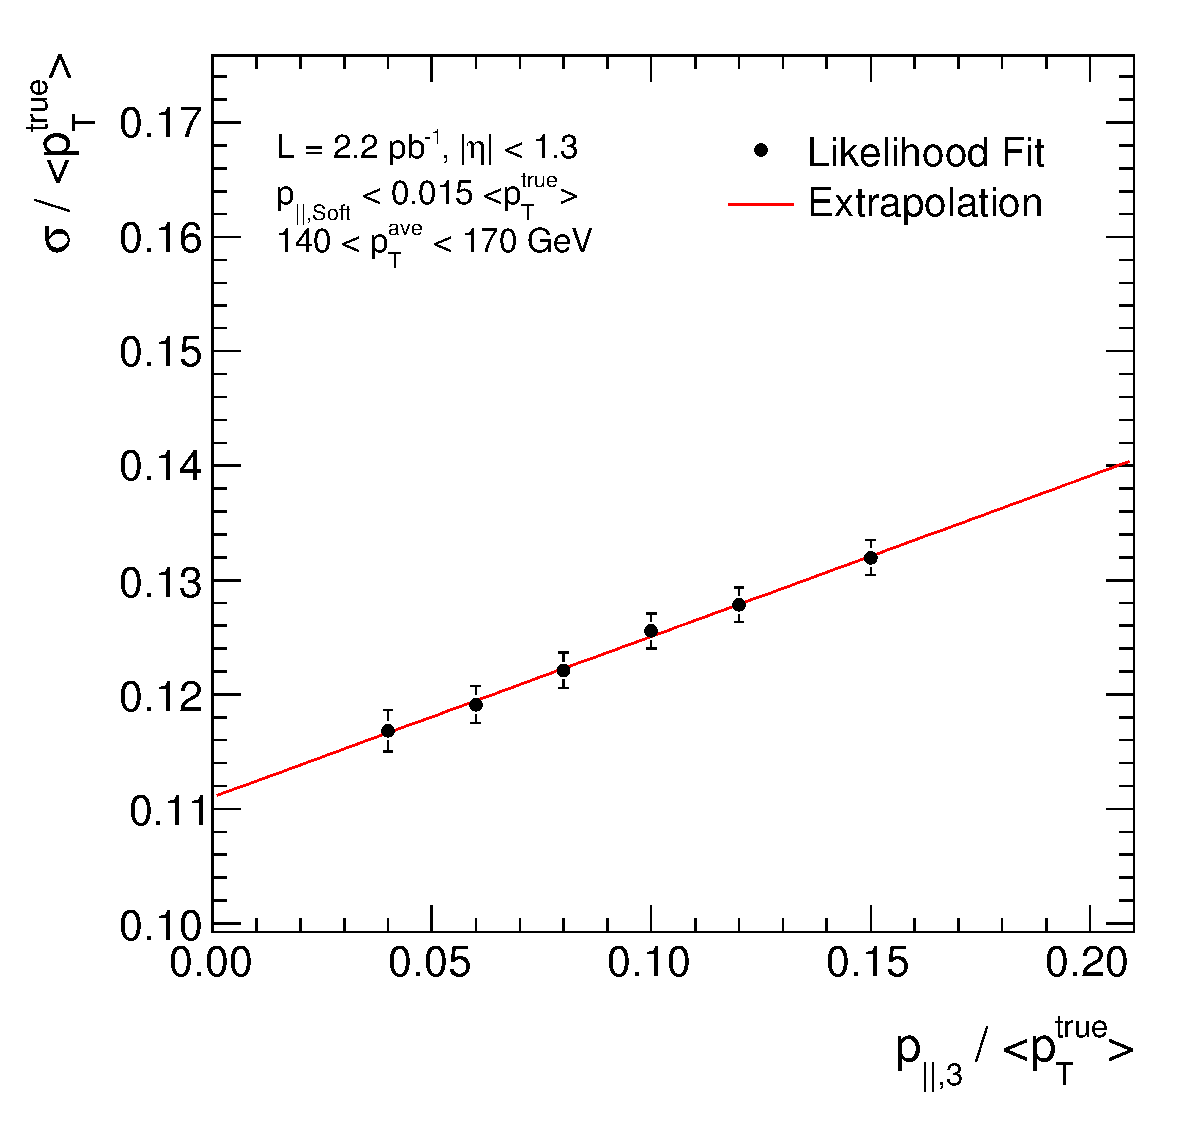
\includegraphics[width=0.45\textwidth]{figures/MaxLike_Data132440-144011_Eta00-13_ExtrapolatedPar0_PtBin4}\\
  \end{tabular}
  \caption{(\textit{Left}) Definition of the dijet axis $\phi_{||}$, the direction normal to the
    angle bisector of the leading two jets in the transverse plane.
    Additional jets with \pt components along $\phi_{||}$ will cause
    a \pt imbalance of the particle jets and bias the measured
    resolution towards larger values.
    (\textit{Right}) Gaussian resolutions \mbox{$\sigma/\mean{\pttrue}$} measured with the unbinned
    fit in Collider data for \mbox{$140 < \ptave < 170\gev$} and different \ppi{3}
    thresholds after suppression of additional soft jet activity along
    $\phi_{||}$. 
    \mbox{$\sigma/\mean{\pttrue}$} on \ppi{3} is linearly
    extrapolated to the case of an ideal dijet event.
  }
\end{figure}

In the following, the statistical uncertainty on the fitted $y$ axis
intercept is used as statistical uncertainty of the measured resolution.
Due to the selection requirement~\qeq{eq:ResFit:ThirdJetSelection},
all events selected for a particular value of the threshold $z$ are
also included in the samples selected with larger values of $z$.
Hence, the measured resolutions in one \ptave bin are strongly correlated.
This correlation is not considered in the quoted uncertainties yet.

The need for compensating the influence of additional jet activity is
the reason why a mean, \pt independent Gaussian the resolution is
measured per \ptave bin.
In that case there is only one free parameter, $\sigma$, which can be
extrapolated straight forward.
Was the response instead parameterised with a \pt dependent function,
e.g. a Gaussian with width
\begin{equation*}
  \sigma\left(\pt\right) = \frac{a}{\pt} \oplus \frac{b}{\sqrt{\pt}}
  \oplus c \;,
\end{equation*}
the parameters $a$, $b$, and $c$ are correlated.
In that case it is not clear how the extrapolation should be performed.

The contribution due to out-of-cone effects to the bias is small, of
the order of $1\%$, as shown in
\qsubfig{fig:ResFit:AddJets:Bias}{left}.
Hence, this bias is corrected for using the MC simulation:
The width of the \ptgen asymmetry, $\sigma(A^{\text{gen}})$, is determined for the
 case of perfectly balanced dijet events, using the
same extrapolation technique as above.
The extrapolated jet \pt resolution is then corrected by 
subtracting $\sqrt{2}\cdot\sigma(A^{\text{gen}})$ in quadrature.

